\chapter{\textit{Data Warehouse}} 


\textit{Data Warehouse} é uma base de dados que armazena suas informações de maneira orientada a satisfazer solicitações de tomadas de decisão \cite{chaudhuri1997}. A diferença entre um típico banco de dados transacional e um  \textit{Data Warehouse}, porém, consiste na maneira como esses dados são armazenados. Em vez de existirem múltiplos ambientes de decisão operando de forma independente, o que com frequência traz informações conflituosas, um \textit{Data Warehouse} unifica as fontes de informações relevantes, de maneira que a integridade  qualidade dos dados são garantidas. \cite{neeraj_sharma_2011}. Dessa forma,\citeonline{chaudhuri1997} afirma que o ambiente de \textit{Data Warehousing} possibilita que seu usuário realize buscas complexas de maneira mais amigável diretamente em um só ambiente, em vez de acessar informações através de relatórios gerados por especialistas. 

\section{Ciclo de vida de um \textit{Data Warehousing}}

\citeonline{Inmon2002} descreve que o \textit{Data Warehouse} é uma coleção de dados que tem como característica ser orientada a assunto, integrada, não volátil e temporal. Por dados orientados a assunto, podemos entender que... . O fato do ambiente ser integrado remete ao fato dele ser alimentado com dados que têm como origem de múltiplas fontes, integrando esses dados de maneira a construir uma única orientação. Como um conjunto não volátil e temporal de dados, é entendido que a informação carregada remete a um determinado momento da aplicação, possibilitando assim acesso a diferentes intervalos de tempo, não havendo como modificá-los atualizando em tempo real.

\subsection{\textit{Extraction-Transformation-Load}}

 Para alcançar as características descritas, o ambiente de Data Warehousing segue o processo que consiste na extração, transformação e carga dos dados, conhecido como \textit{Extraction-Transformation-Load} (ETL). Cada um dos passos recebe a seguinte descrição:

\begin{easylist}[itemize]

	& \textbf{Extração: } Primeira etapa do processo de ETL, consiste na leitura e entendimento da fonte 		dos dados, copiando os que são necessário para futuros trabalhos \cite{Kimball2002}.  
	& \textbf{Transformação: } Após a etapa de extração ter sido feita, os dados podem receber diversos tipos de transformações, que incluem correções de conflitos, conversão de formatos, remoção de campos que não são úteis, combinação entre dados de diversas fontes, entre outros \cite{Kimball2002}.
	& \textbf{Carga: } Após ter sido realizado o processo de transformação, os dados já estão prontos para serem carregados no \textit{Data Warehouse}, tornando possível que todos os dados visualizados após esse processo reflitam a informação que passou pelos processos de extração e transformação \cite{neeraj_sharma_2011}.  

	\end{easylist}

A figura  descreve a arquitetura de um ambiente de \textit{Data Warehousing}, envolvendo os três processos citados anteriormente

\section{Modelagem Dimensional}

\citeonline{Kimball2002} afirma que a habilidade de visualizar algo tão abstrato como um conjunto de dados  de maneira concreta e tangível é o segredo da compreensibilidade, de modo que um modelo de dados que se inicia de forma simples tende a ser simples até o final da modelagem, ao contrário de um modelo que já se inicia de forma complicada. Nesse contexto, o modelo dimensional difere em muitos aspectos do modelo normalizado em sua terceira forma normal, também conhecido como modelo entidade-relacionamento. O modelo normalizado contém seus dados divididos em muitas entidades, cada qual identificada como uma tabela, buscando assim evitar redundância entre os dados, sendo eles armazenados em tempo real na medida que forem atualizados. O problema associado a essa solução é a tamanha complexidade adquirida pelos modelos, uma vez que são criadas um número grande de tabelas dificultando assim sua navegação. Em um sentido oposto, a modelagem dimensional resolve esse problema associado à complexidade, uma vez que, mesmo possuindo as mesmas informações que um modelo normalizado, elas estão modeladas de forma que estejam em sintonia com o entendimento do usuário e ao alto desempenho de consultas. 

Um modelo dimensional é composto por tabelas fatos e tabelas dimensões, que quando juntas formam o esquema estrela. A tabela fato é a tabela primária no modelo dimensional. O termo \textit{fato} está associado à maneira como ela representa uma medida de negócio \cite{Kimball2002}. Já a tabela dimensão contém descrições textuais dos negócios envolvidos, o que a torna a chave para que o modelo seja utilizável e de fácil entendimento. \citeonline{Kimball2002} faz uma relação direta entre a qualidade do Data Warehouse como um todo e a qualidade e profundidade dos atributos das tabelas dimensão. O esquema estrela, já definido como a união entre tabelas fato e dimensão, pode ser representado da forma como o exemplo da figura \ref{fig:estrela} descreve:
 
\begin{figure}[h!]
\centering
\includegraphics[keepaspectratio=false,scale=0.50]{figuras/figuras_matheus/star.eps}
\caption{Esquema estrela extraído de \citeonline{valeria2012}}
\label{fig:estrela}
\end{figure}
\FloatBarrier
 
\subsection{OLAP \textit{On-Line Analytic Processing}}

A atividade que consiste em buscar e apresentar os dados de um \textit{Data Warehouse}, sendo essa busca quase sempre baseada em um cubo multidimensional de dados, é chamada de \textit{On-Line Analytic Processing} (OLAP) \cite{Kimball2002}. A consulta OLAP difere da consulta do tipo \textit{On-Line Transaction Processing} (OLTP) pelo fato dos seus dados terem passado por um processo de ETL, de modo que sua performance foi melhorada para uma análise mais fácil e rápida, enquanto na consulta do tipo OLTP o sistema foi modelo de modo a capacitar inserções, atualizações e remoções de dados obedecendo regras de normalização. A tabela \ref{tab:hilmer} evidencia as diferenças entre aplicações OLTP e OLAP extraídas do trabalho de \citeonline{hilmer2002}: 

\begin{table}[!ht]
	\begin{center}
	
	\input{tabelas/tabelasMatheus/hilmer_olap_oltp.ltx} 
	\caption{Diferenças entre OLTP e OLAP extraídas de \cite{hilmer2002}}
	\label{tab:hilmer}
	\end{center}
	\end{table}	
	\FloatBarrier	

	





